\documentclass[12pt,a4paper,oneside]{article}
\usepackage[colorlinks=true, unicode]{hyperref}
\usepackage[utf8]{inputenc}
\usepackage[czech]{babel}
\usepackage{graphicx}
\usepackage{pdfpages}
\textwidth 16cm \textheight 25cm
\topmargin -1.3cm 
\oddsidemargin 0cm
\usepackage{footnote}
\pagestyle{empty}
\begin{document}
\title{Nízkošumový předzesilovač LNA01A}
\author{Jakub Kákona, kaklik@mlab.cz}
\maketitle

\thispagestyle{empty}
\begin{abstract}
Vstupní nízkošumový zesilovač určený k pásmovému zesílení signálu bezprostředně za anténou. Je optimalizovaný na velmi nízký šum, aby umožnil konstrukci přijímacích sestav s malým šumovým číslem.  
\end{abstract}

\begin{figure} [htbp]
\begin{center}
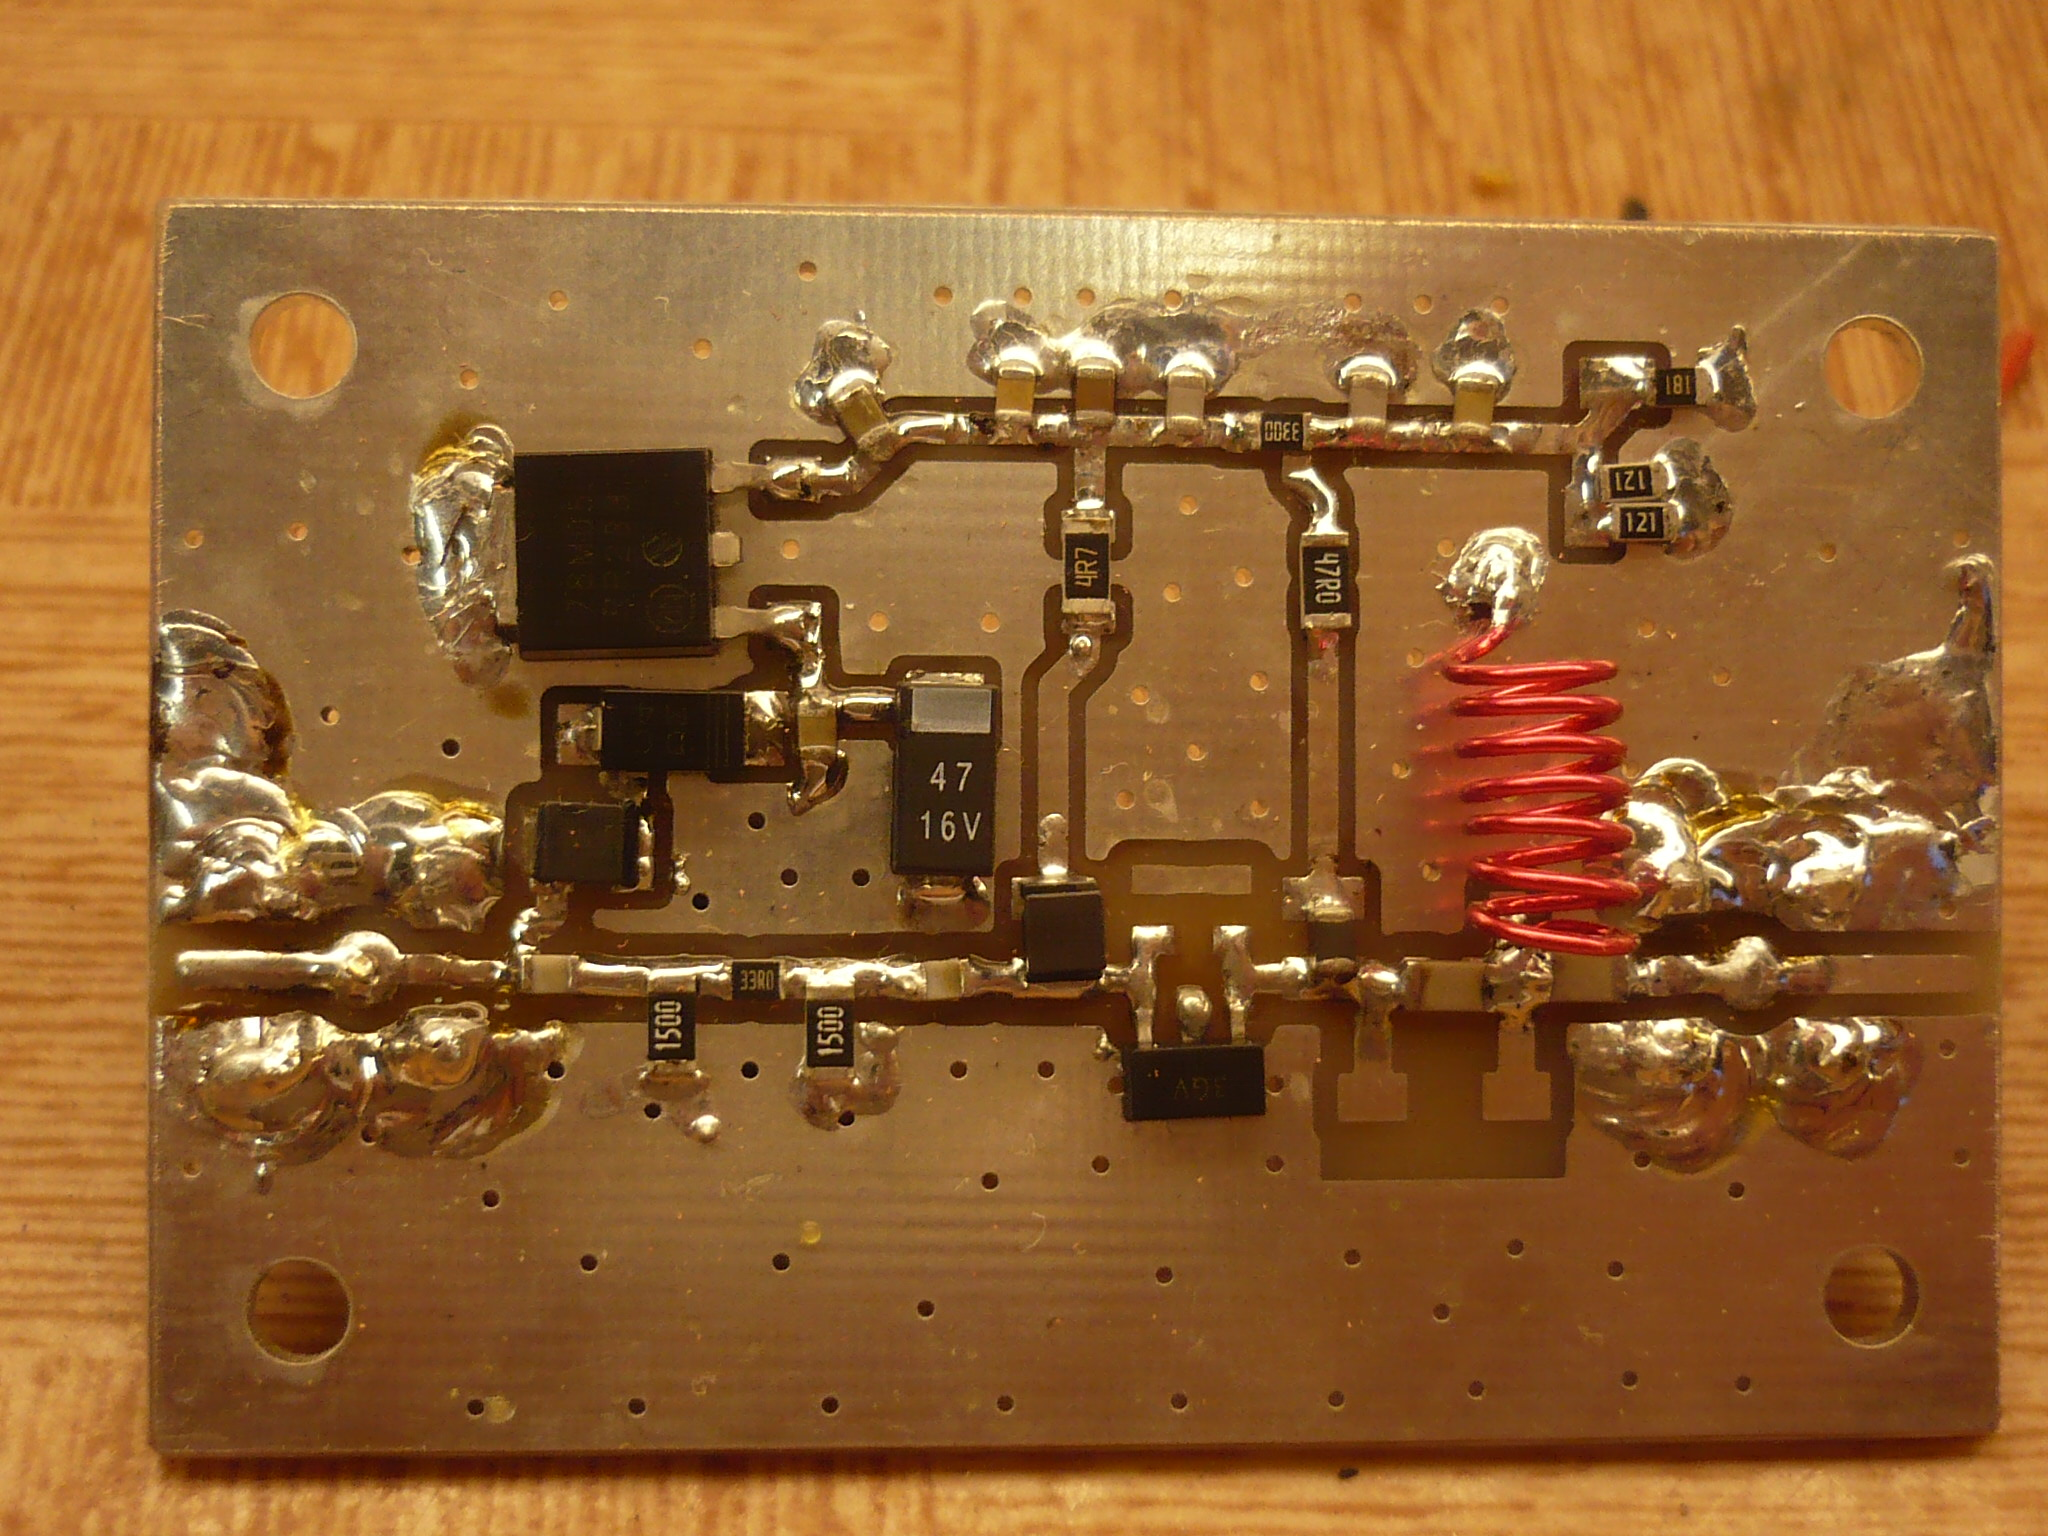
\includegraphics [width=80mm] {../img/LNA01A_bottom_big.jpg} 
\end{center}
\end{figure}

\begin{figure} [b]

\includegraphics [width=25mm] {../img/LNA01A_QRcode.png} 
\end{figure}

\newpage
\tableofcontents


\section{Technické parametry}
\begin{table}[htbp]
\begin{center}
\begin{tabular}{|c|c|p{4.7cm}|}
\hline
\multicolumn{1}{|c|}{Parametr} & \multicolumn{1}{|c|}{Hodnota} & \multicolumn{1}{|c|}{Poznámka} \\ \hline
Napájecí napětí & do +12V &  max 200mA \\ \hline
Frekvenční rozsah  & 100 - 200 MHz & Při osazení jinými součástkami i 450MHz \\ \hline
Maximální RF vstupní výkon  & + 24 dBm & Maximálně 1V na RF input \\ \hline
OIP3  & 40dBm &  \\ \hline
Šumové číslo  & $<$ 0.8 dB & \\ \hline
\end{tabular}
\end{center}
\end{table}


\section{Popis konstrukce}

\subsection{Zapojení}

Zapojení zesilovače je realizováno na plošném spoji materiálu FR4. Plošný spoj je možné osadit přímými SMA konektory, nebo konektory na hranu desky. 

Zapojení modulu je následující

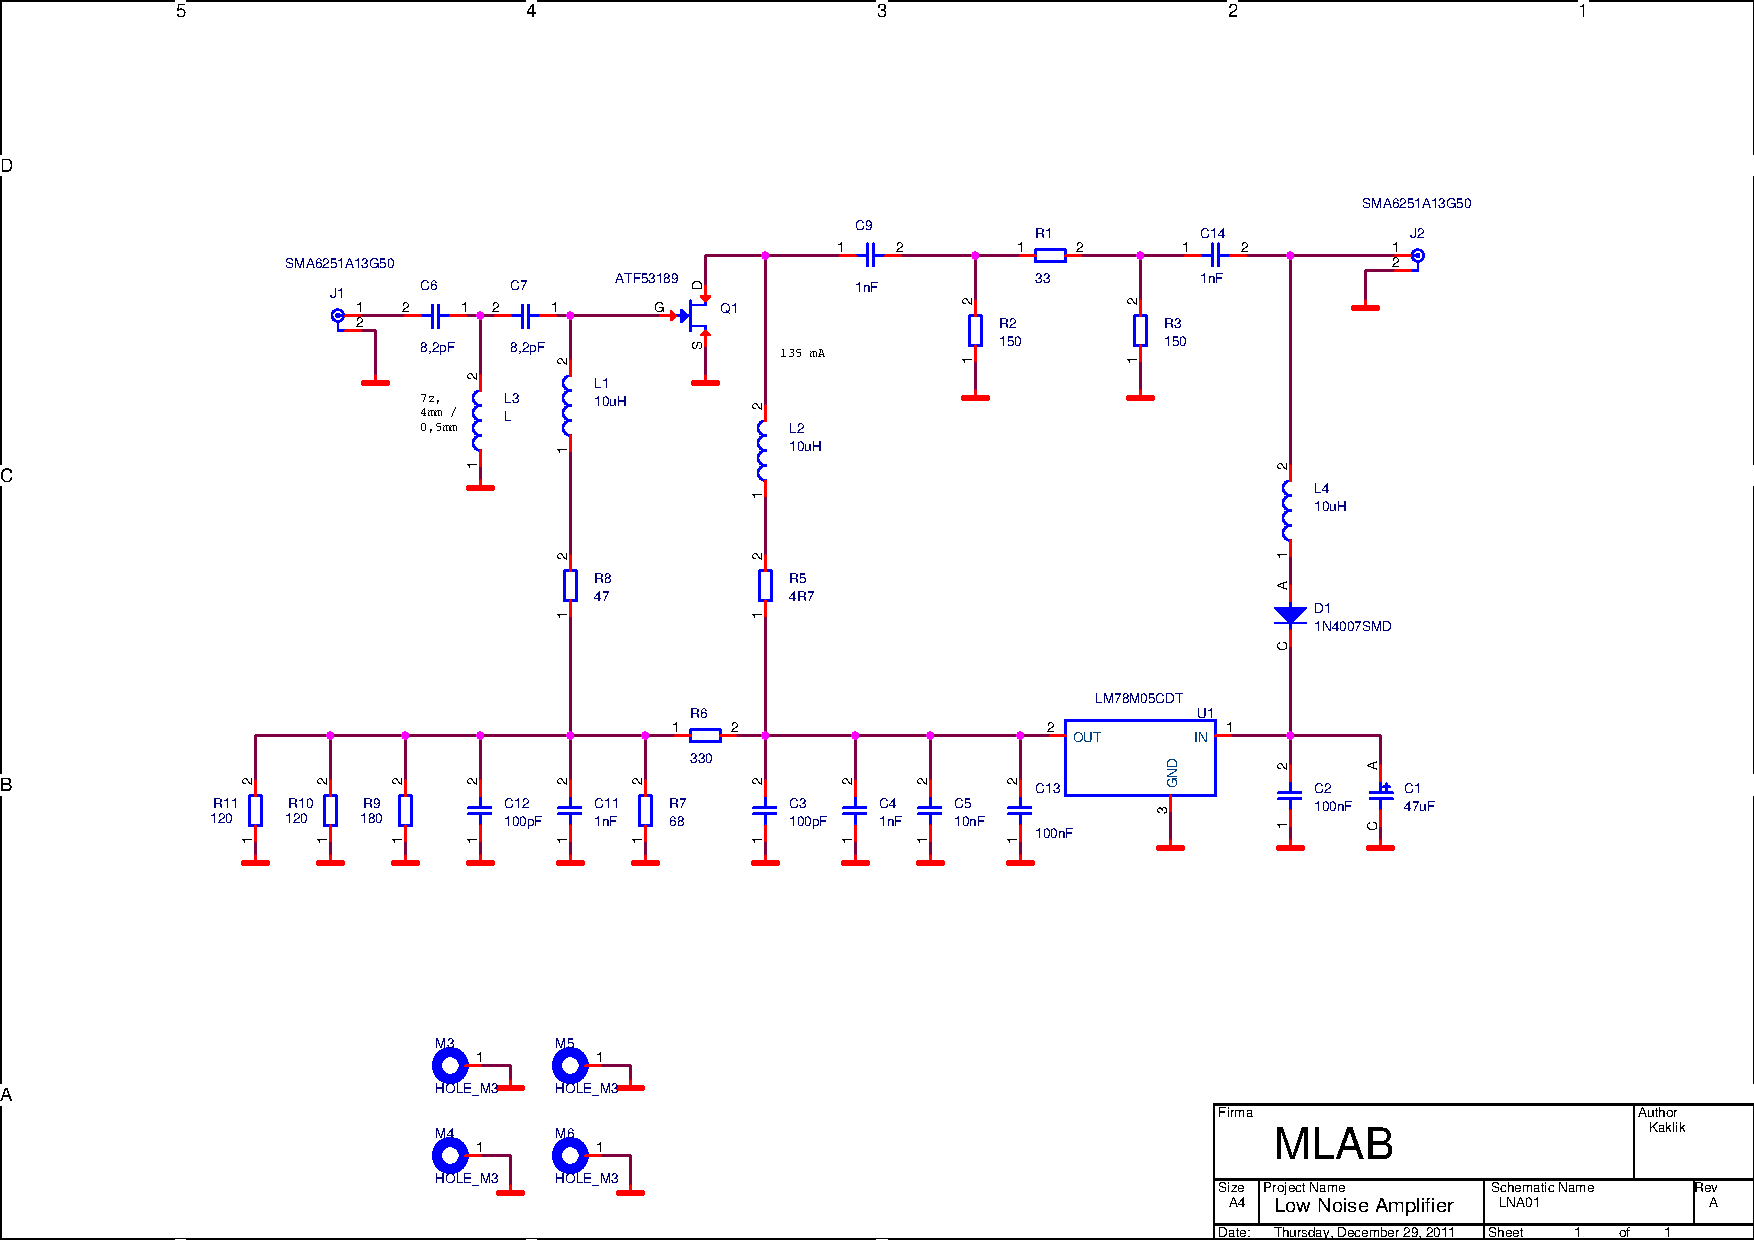
\includepdf[pages={1},landscape=true]{../../sch/LNA.pdf}


\subsection{Odrušení}

Zesilovač musí být nutně umístěn v plechové stínící krabičce, aby nemohlo dojít k jeho rozkmitání signálem vyzařovaným do antény. Taktéž kovová krabička zabezpečuje vyšší kvalitu signálu na výstupu zesilovače. 

\subsection{Mechanická konstrukce}

U zesilovače se předpokládá jeho umístění do plechové pocínované stínící krabičky ve které je zesilovač zaletován za konektory. 
Otvory pro konektory se do krabičky vytváří lochovacími kleštěmi s průměrem nástroje 6.35mm.  Pro lochování děr je vytvořena šablona \textit{hole\_pattern.pdf}

\section{Výroba a testování}

Osazování SMD součástek probíhá do tavné pasty, včetně tranzistoru. V případě osazování tranzistoru je potřeba věnovat zvýšenou pozornost antistatické ochraně, kterou je nutné zabezpečit nepoškození tranzistoru. Tranzistor může být letován pouze elektrostaticky bezpečnými nástroji, jako je horkovzduch nebo IR pájka. 
Vzduchová cívka se neosazuje do doby plného osazení a zaletování SMD součástek. 

Po zaletování SMD součástek lze zaletovat vzduchovou cívku, která může být letována i kontaktní pájkou. Je vhodné využít pájku o vyšším výkonu, aby bylo možné cívku kvalitně zaletovat k zemní ploše. 

Následně po úplném zaletování cívky je možné odzkratovat, vstup a výstup zesilovače. Ten je zkratovaný od výroby PCB neodleptanou vrstvou mědi na opačné straně, než jsou SMD součástky. Na místě vstupního a výstupního konektoru je proto potřeba odhranit otvor pro střed SMA konektoru. To lze nejlépe provést vrtákem o průměru přibližně 8mm. 

\subsubsection{Osazení}

Trimr P1 se neosazuje, místo toho je nahrazen kombinací rezistorů R9, R10 a R11, které jsou osazeny na jeho pozici. Osazení rezistorů na místo trimru je vidět na obrázku \ref{osazeni}.


\begin{figure} [htbp]
\begin{center}
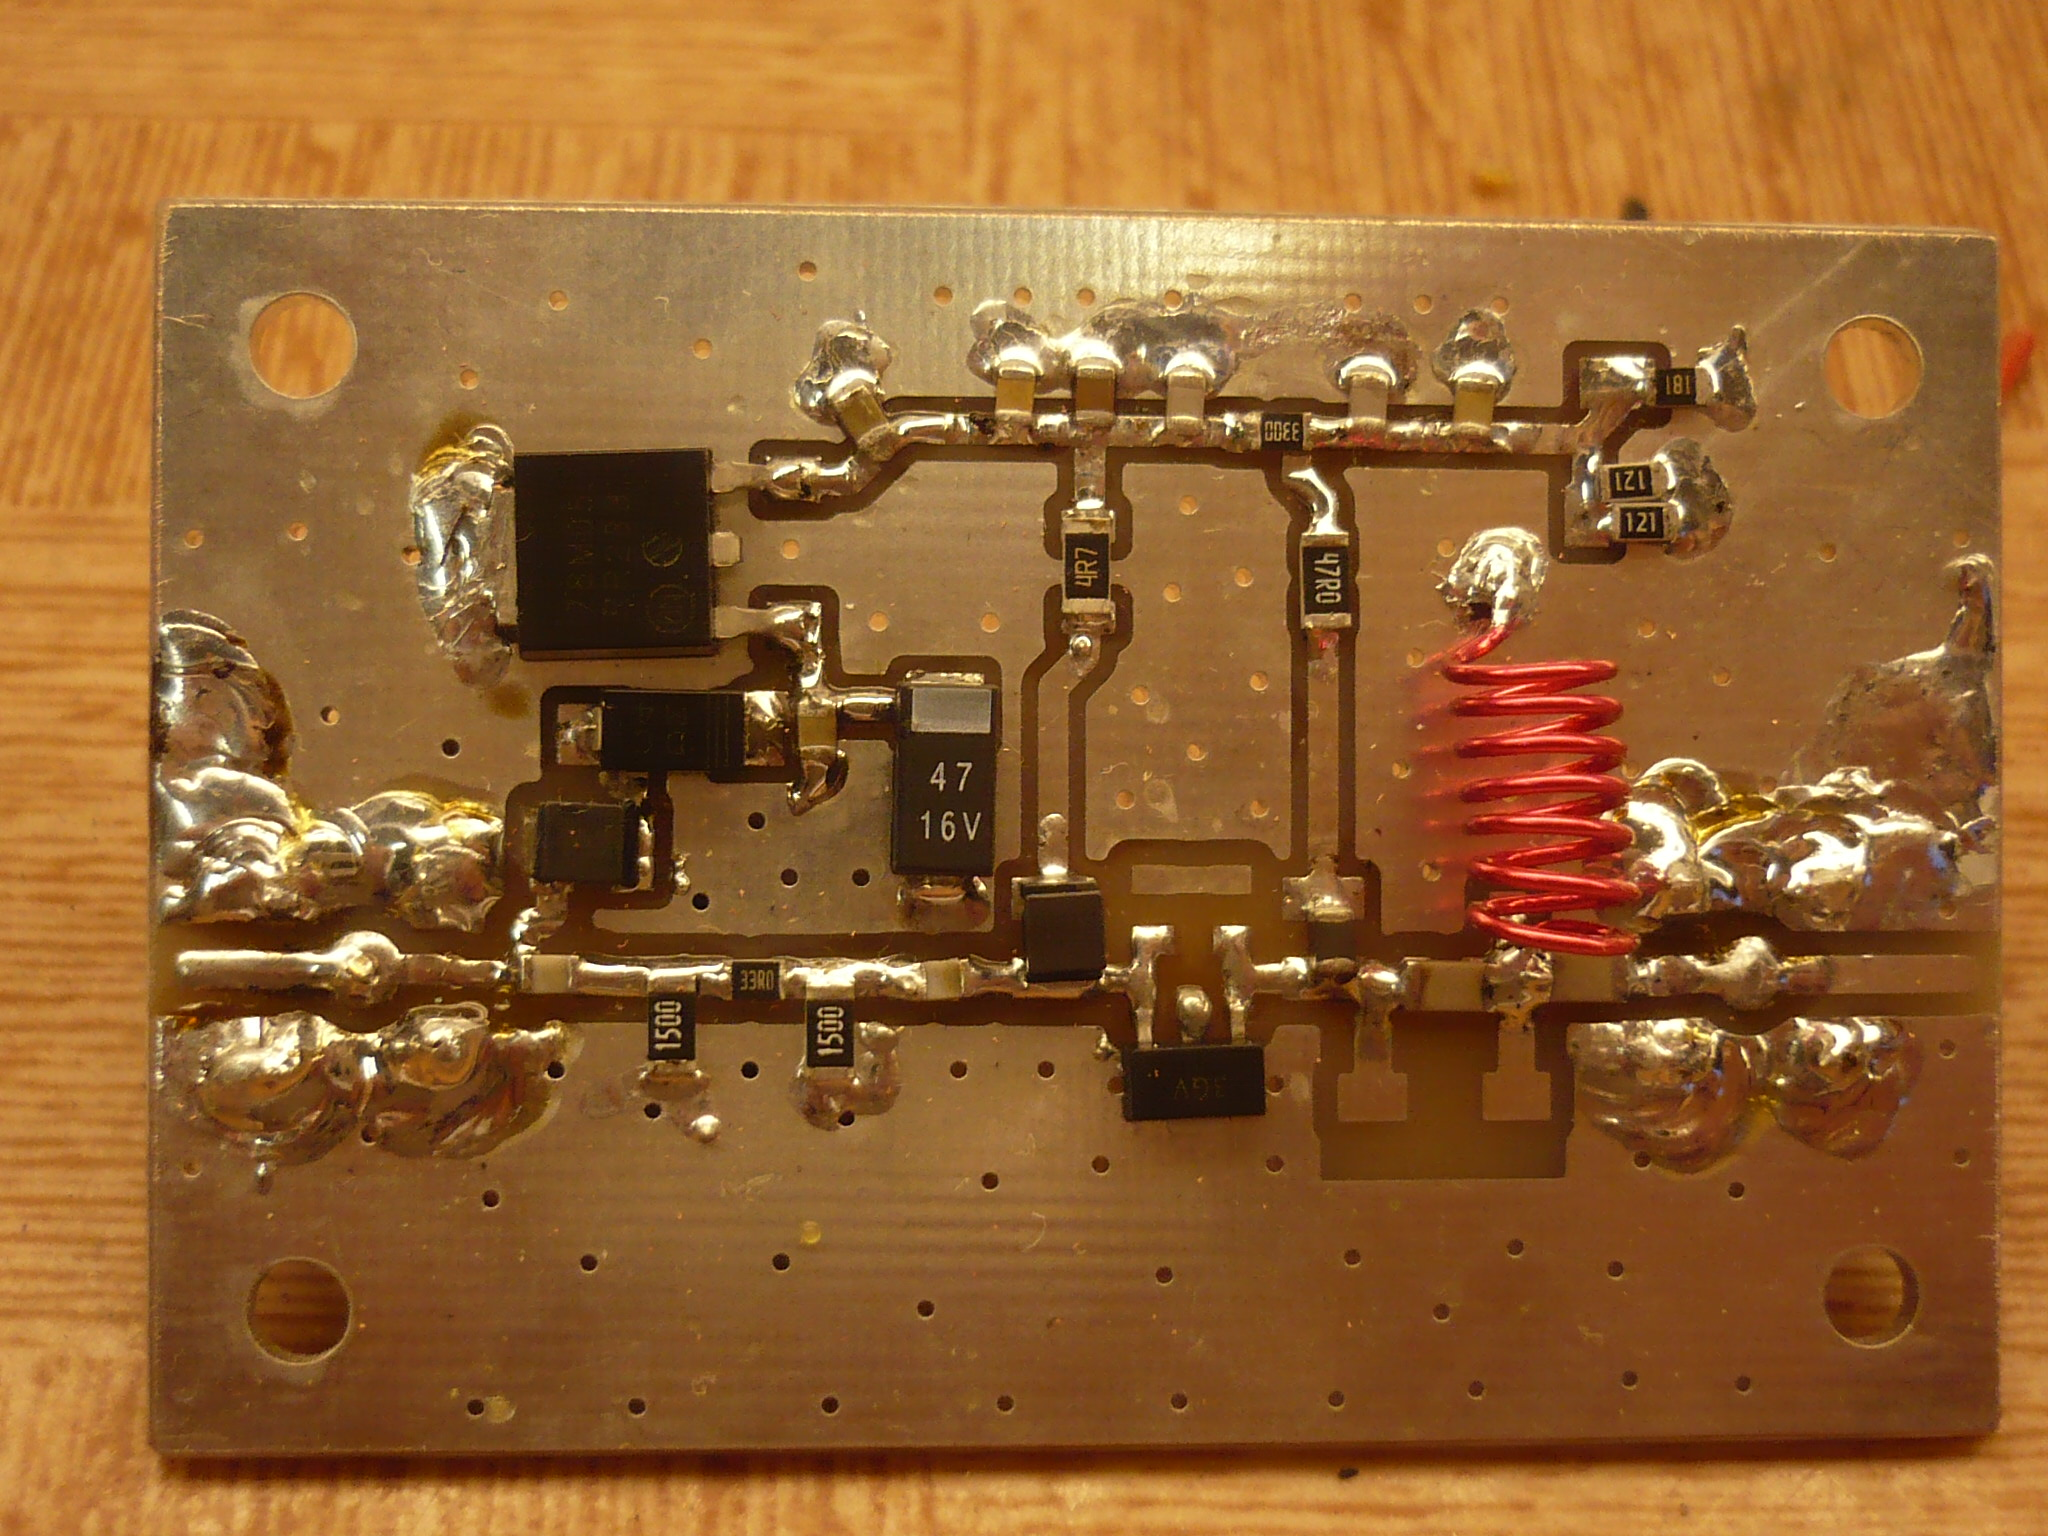
\includegraphics [width=130mm] {../img/LNA01A_bottom_big.jpg}
\caption{Fotografie osazení rezistorů na místo trimru.}
\label{osazeni}
\end{center}
\end{figure}


Vzduchová cívka L3 pro naladění na 143 MHz vychází 7 závitů z měděného drátu průměru 0,5 mm motáno na průměr tyčky 4mm (vrták). Cívka je roztažená tak jak je vidět na fotografii. Kondenzátory C1 a C2 jsou 8,2 pF. Zpětná vazba u LNA není potřeba, pouze zvyšuje šumové číslo a snižuje zisk asi o 1dB. Trim je nahrazen odporem 45 $/Omega$ a celkový proud celým LNA by měl být kolem 153mA, potom je proud Source tranzistoru asi 135mA. 

\newpage


\begin{figure} [h!tbp]
  \centering
  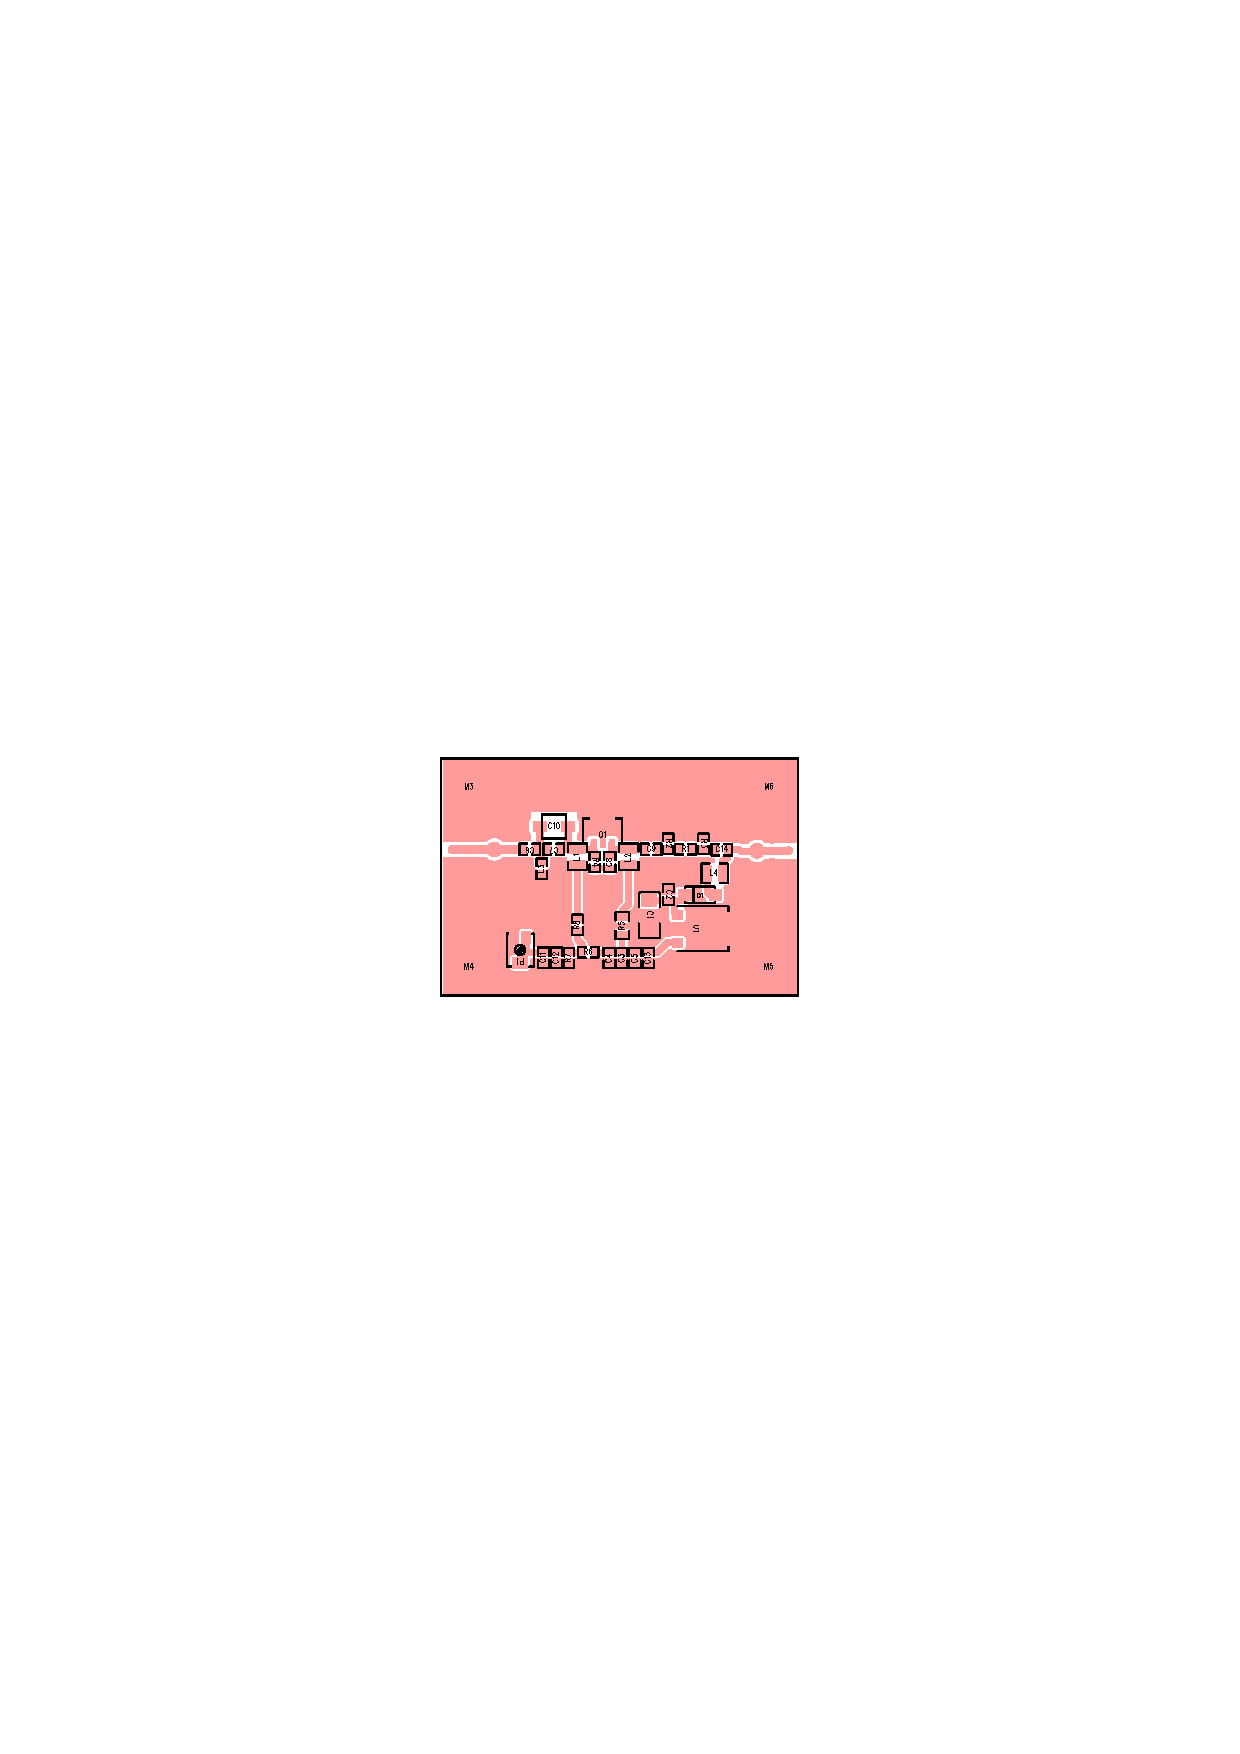
\includegraphics[trim = 7.3cm 12.7cm 7.3cm 12.7cm, clip, width=6.5cm]{../../hw/cam_doc/O1.pdf}
  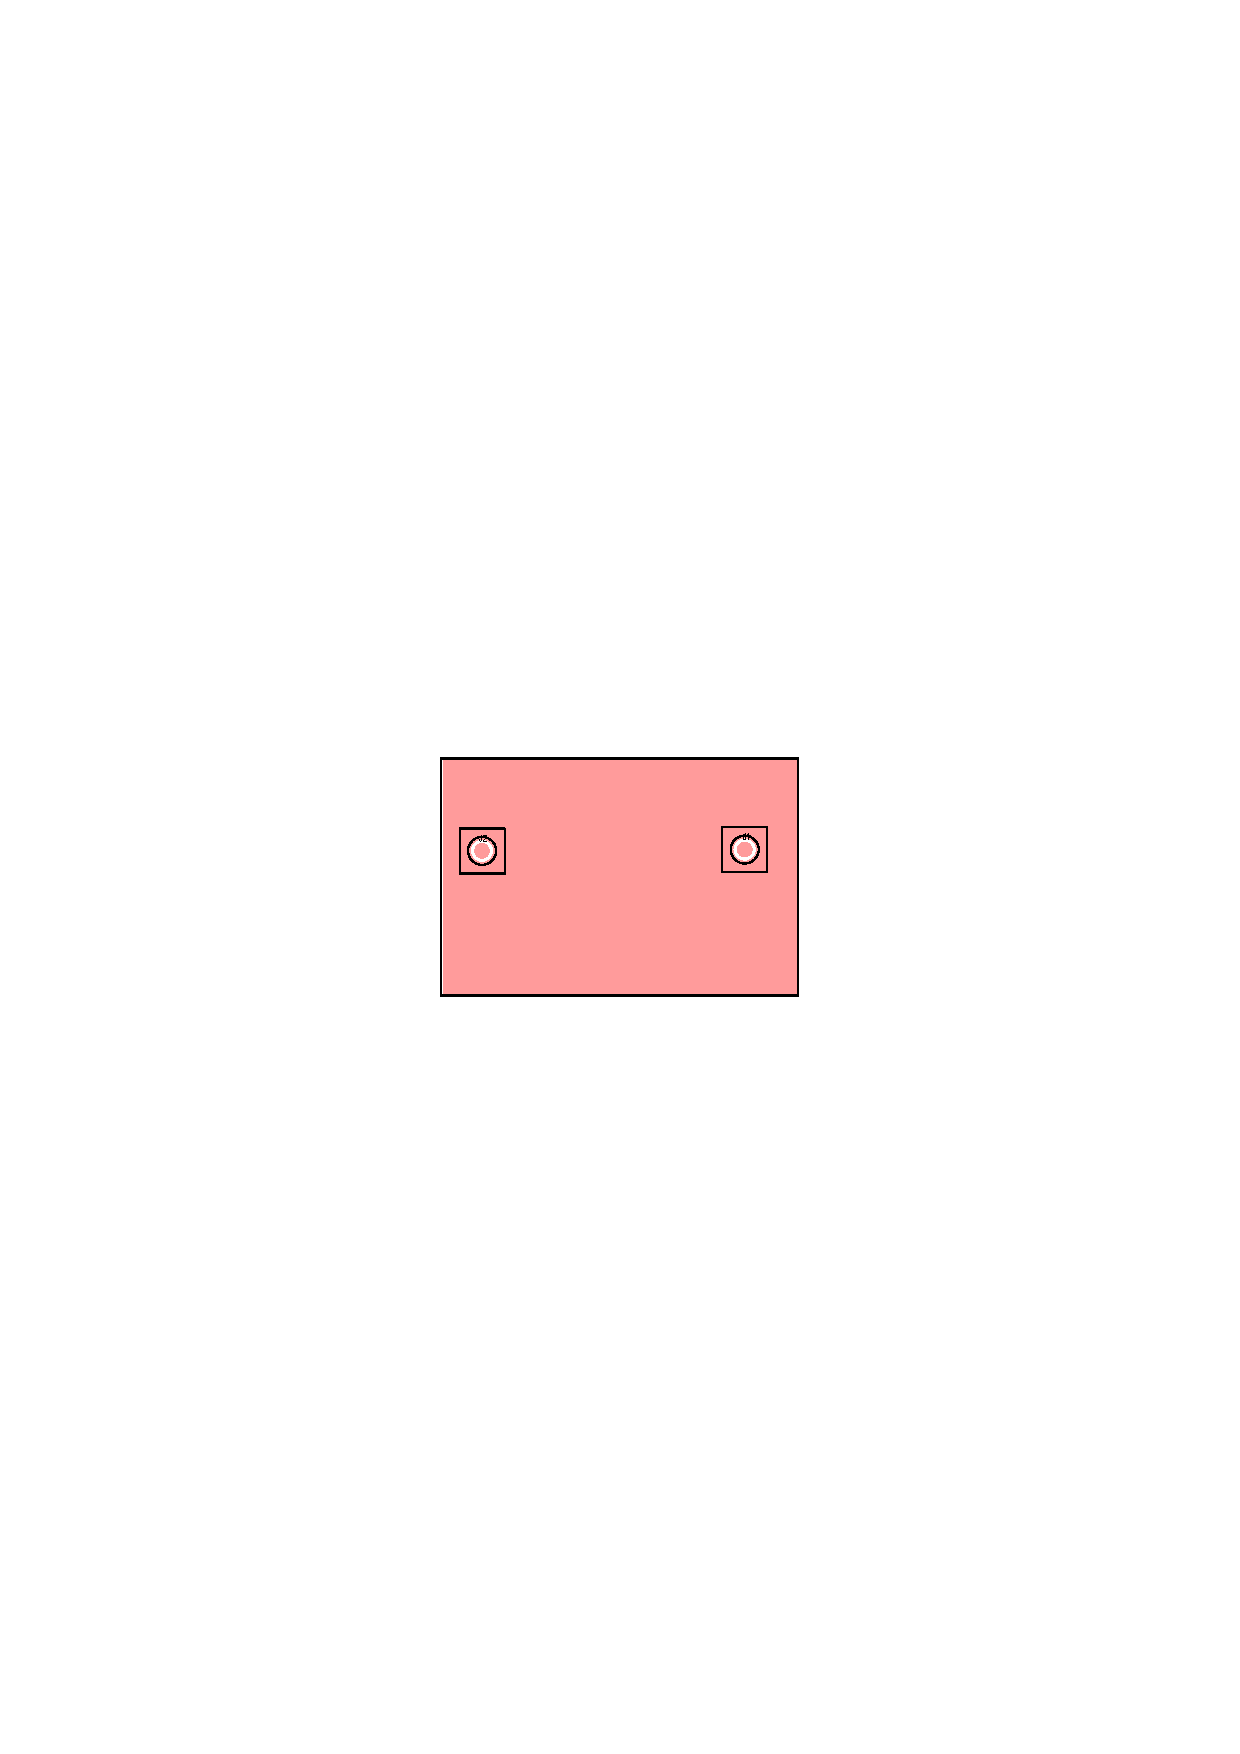
\includegraphics[trim = 7.3cm 12.7cm 7.3cm 12.7cm, clip, width=6.5cm]{../../hw/cam_doc/O2.pdf}
  \caption{Osazovací plán horní a spodní strany plošného spoje}
  \label{fig:osazovaci_plan}
\end{figure}

\begin{savenotes}
\begin{table}[h!]
\begin{center}
\begin{tabular}{ |c|c|c|c| }
\hline 
Počet & Označení & Typ  & Pouzdro  \\ 
\hline 
1	&	C1	&	47uF	&	ELYT-C	\\
2	&	C2,C13	&	100nF	&	C0805	\\
2	&	C3,C12	&	100pF	&	C0805	\\
5	&	C4,C9,C11,C14	&	1nF	&	C0805	\\
1	&	C8	&	-	&		\\
1	&	C5	&	10nF	&	C0805	\\
1	&	C6	&	8,2pF	&	C0805	\\
1	&	C7	&	5,6pF	&	C0805	\\
1	&	C10	&	5pF	&	C0805	\\
1	&	D1	&	M4	&	SMA	\\
2	&	J1,J2	&	SMA6251A13G50	&		\\
3	&	L1,L2,L4	&	10uH 160mA	&	L1812	\\
1	&	L3	&	L	&	7x 0.5mm 4mm	\\
1	&	P1	&	-	&		\\
1	&	Q1	&	ATF53189	&	SOT89	\\
1	&	R1	&	33	&	R0805	\\
2	&	R2,R3	&	150	&	R0805	\\
1	&	R4	&	-	&		\\
1	&	R5	&	4R7	&	R1206	\\
1	&	R6	&	330	&	R0805	\\
1	&	R7	&	68	&	R0805	\\
1	&	R8	&	47	&	R0805	\\
1	&	R9	&	180	&	R0805	\\
1	&	R10,R11	&	120	&	R0805	\\
1	&	U1	&	LM78M05CDT	&	TO252	\\
\hline 
\end{tabular}
\end{center}
\caption{Seznam součástek pro osazení plošného spoje.}
\label{seznam_soucastek}
\end{table}
\end{savenotes}

\newpage



\subsubsection{Nastavení}

Dolaďování předzesilovače se provádí deformací vzduchové cívky. Kmitočtovou charakteristiku zesilovače lze přeměřit přístrojem sestaveným z modulů MLAB. Je k tomu potřeba SDR-widget s přijímačem SDRX01B a šumový generátor.

Protože zmíněný generátor šumu má pro účely měření v podstatě plochou frekvenční charakteristiku, tak můžeme bez kalibrace jeho výstup připojit přímo na LNA.

Součástí PySDR je detekční skript, který umožňuje přijímač přelaďovat přes zvolené frekvenční pásmo a zaznamenávat amplitudu signálu. Tento skript může být spuštěn několika způsoby, které se liší jednak podle toho, jestli chceme spustit měření v PySDR, nebo samostatně.


\begin{thebibliography}{99}
\bibitem{DR2G}{Původní konstrukce} 
\href{http://}{Původní konstrukce LNA}

\end{thebibliography}
\end{document}